% !TeX program = xelatex
\documentclass[9pt]{beamer}
\usepackage{xcolor}
\definecolor{orange}{HTML}{FF1053}
\definecolor{lightgray}{HTML}{CCCCCC}
\definecolor{red}{HTML}{AC454A}
\definecolor{brown}{HTML}{EAD296}
\definecolor{darkgrey}{HTML}{313630}
\definecolor{cornflower}{HTML}{247BA0}
\definecolor{sienna}{HTML}{6C464F}
\usefonttheme{professionalfonts} % using non standard fonts for beamer
\usefonttheme{serif} % default family is serif
\usepackage{fontspec}
\usepackage{setspace}
\usepackage{natbib}
\usepackage{animate}
\usepackage{graphicx}
\usepackage{algorithm2e}
%\usepackage[T1]{fontenc}

\bibliographystyle{abbrv}
%\setmainfont{Liberation Serif}
%\setmainfont{Liberation Serif}
\setmainfont{Comfortaa}
%\usepackage[T1]{fontenc}

\setbeamercolor{frametitle}{bg=orange,fg=white}
\setbeamercolor{author in head/foot}{bg=orange,fg=white}

%\setbeamerfont{page number}{size=\Huge}

%\setbeamertemplate{itemize itemjpegs}[circle]
\useinnertheme{circles}
\setbeamercolor{palette primary}{bg=orange,fg=white}
%\setbeamercolor{palette secondary}{bg=red,fg=white}
\setbeamertemplate{itemize item}{\color{darkgrey}$\circ$}
\setbeamercolor{structure}{fg=darkgrey} % itemize, enumerate, etc

%\setbeamercolor{section in head/foot}{bg=red}
\setbeamercolor{title}{fg=orange} %, bg=brown
\setbeamercolor{author}{fg=darkgrey}
\setbeamercolor{institute}{fg=darkgrey}
\setbeamercolor{date}{fg=darkgrey}
%\setbeamercolor{normal text}{fg=darkgrey}
\makeatletter
\setbeamertemplate{headline}{%
	\usebeamercolor[bg]{frametitle}\rule{\textwidth}{1cm}
}
\setbeamerfont{title}{size=\LARGE}
\setbeamerfont{institute}{size=\normalsize}
\renewcommand*{\bibfont}{\scriptsize}


\setbeamertemplate{frametitle}{%
	\vskip-1cm%
	\begin{minipage}[c][\headheight][c]{\textwidth}%
		\usebeamerfont{frametitle}
		\strut\insertframetitle\par
		{%
			\ifx\insertframesubtitle\@empty%
			\else%
			{\usebeamerfont{framesubtitle}\usebeamercolor[fg]{framesubtitle}\strut\insertframesubtitle\par}%
			\fi
		}%      
		\vspace*{0.05cm}
	\end{minipage}%
	\vskip-0.1em
}
%\setbeamertemplate{footline}{%
%	\leavevmode%
%	\hbox{\begin{beamercolorbox}[wd=\paperwidth,ht=4.5ex,dp=3.125ex]{author in head/foot}%
%			\usebeamerfont{author in head/foot} bar
%	\end{beamercolorbox}}%
%	\vskip0pt%
%}
\makeatother


\title{Simulation-based Inference \\
	\small Inverting Simulators}
\author{Talk by Stefan Wezel}
\institute{mlcolab @ Tübingen University Cluster of Excellence}
\date{\today}


%\setbeamertemplate{sidebar right}{}
%\setbeamertemplate{footline}{%
%	\hfill\usebeamertemplate***{navigation symbols}
%	\hspace{1cm}\insertframenumber{}}
\setbeamerfont{page number in head/foot}{size=\small}
    \setbeamertemplate{footline}{%
	\raisebox{5pt}{\makebox[\paperwidth]{\hfill\makebox[10pt]{\scriptsize\insertframenumber}}}}
\setbeamertemplate{navigation symbols}{}
%\onehalfspacing
\setstretch{1.3}
\begin{document}
	

\setbeamercolor{background canvas}{bg=white}
\setbeamercolor{normal text}{fg=darkgrey}
\usebeamercolor[fg]{normal text}
\begin{frame}[plain]
	\titlepage
\end{frame} 



\setbeamercolor{background canvas}{bg=white}
\setbeamercolor{normal text}{fg=darkgrey}
\usebeamercolor[fg]{normal text}
\setbeamertemplate{itemize item}{\color{darkgrey}$\circ$}
\begin{frame}
\frametitle{Overview}
\framesubtitle{}
\begin{itemize}
	\item The problem setting %(as this is rather unfamiliar to ML researchers)
	\item Traditional approaches and their issues
	\item Using Neural Nets to alleviate them
	\item A worked example
	\item Outlook %(and some advertisement)
\end{itemize}
\end{frame} 






\begin{frame}
\frametitle{What and Why?}
\framesubtitle{An Example}
\begin{itemize}
	\item Inverting simulators?% - so first let's find out what a simulator is
	\item What is a simulator? % in context of this presentation
	\begin{itemize}
		\item Forward, generative model with parameters and stochasticity
		\item Produces observations
		\item In context of this talk computer program, but can be electrical circuit (Hodgkin–Huxley model)
	\end{itemize}
	\item Used by scientists to model empirical observed data
	\item Used in particle physics, population genetics, epidemiology
	\item Encode knowledge about systems gathered over centuries
%	\item Model for theories developed over centuries
	% For further intuition, let's look at an example (and I'm not gonna talk about epidemiology)
%	\item Imagine you are a physicist
%	\item You have also highly sophisticated experiments that can produce observations
%	\item You have highly sophisticated models, theories that can produce observations like from your experiment, that were developed over centuries
%	\item But what do we actually care about? How do you perform inference?
%	\begin{itemize}
%		\item What were the parameters for your observation
%%		\item In other words: what were the parameters $\theta$ for observation $x_0$
%	\end{itemize}
%	\item You're simulator has no direct answer to this question except for trying everything out
\end{itemize}
\end{frame} 



\begin{frame}
\frametitle{What and Why?}
\framesubtitle{An Example}
	\begin{figure}
	\includegraphics[width=1\linewidth]{figures/lhc1.pdf}
\end{figure}
\tiny Figure derived from \textit{cern.ch, Achintya Rao and Tom McCauley, sciencealert.com}
\end{frame}
\begin{frame}
\frametitle{What and Why?}
\framesubtitle{An Example}
\begin{figure}
	\includegraphics[width=1\linewidth]{figures/lhc2.pdf}
\end{figure}
\tiny Figure derived from \textit{cern.ch, Achintya Rao and Tom McCauley, sciencealert.com}
\end{frame}
\begin{frame}
\frametitle{What and Why?}
\framesubtitle{An Example}
\begin{figure}
\includegraphics[width=1\linewidth]{figures/lhc3.pdf}
\end{figure}
\tiny Figure derived from \textit{cern.ch, Achintya Rao and Tom McCauley, sciencealert.com}
\end{frame} \begin{frame}
\frametitle{What and Why?}
\framesubtitle{An Example}
\begin{figure}
\includegraphics[width=1\linewidth]{figures/lhc4.pdf}
\end{figure}
\tiny Figure derived from \textit{cern.ch, Achintya Rao and Tom McCauley, sciencealert.com}
\end{frame} \begin{frame}
\frametitle{What and Why?}
\framesubtitle{An Example}
\begin{figure}
\includegraphics[width=1\linewidth]{figures/lhc5.pdf}
\end{figure}
\tiny Figure derived from \textit{cern.ch, Achintya Rao and Tom McCauley, sciencealert.com}
\end{frame} \begin{frame}
\frametitle{What and Why?}
\framesubtitle{An Example}
\begin{figure}
\includegraphics[width=1\linewidth]{figures/lhc6.pdf}
\end{figure}
\tiny Figure derived from \textit{cern.ch, Achintya Rao and Tom McCauley, sciencealert.com}
\end{frame} \begin{frame}
\frametitle{What and Why?}
\framesubtitle{An Example}
\begin{figure}
\includegraphics[width=1\linewidth]{figures/lhc7.pdf}
\end{figure}
\tiny Figure derived from \textit{cern.ch, Achintya Rao and Tom McCauley, sciencealert.com}
\end{frame} 



\begin{frame}
\frametitle{What and Why?}
\framesubtitle{Formalizing our Example}
\begin{itemize}
	\item Before we go into SBI, let's take a minute to formalize our setting
	\item Simulator has parameters $\theta$, nuisance parameter $z$ and produces data $\hat{x}$
	\begin{itemize}
		\item It implicitly defines $p(\hat{x},z|\theta)$ (it yields samples from this distribution)
	\end{itemize}
	\item Given a (real) observation $x_0$, we would be interested in the parameters that produced it
	\begin{align}
	p(\theta|x=x_0) = \frac{p(x|\theta)p(\theta)}{p(x)} = \frac{\overbrace{\int p(x,z|\theta)dz}^{intractable} p(\theta)}{\underbrace{\int p(x|\theta)p(\theta)d\theta}_{intractable}},
	\end{align}
%	\begin{itemize}
%		\item $p(\theta|x_0)$ -> posterior over parameters
%		\item In simple cases, we could apply Bayes' rule and compute it analytically
%		\item What is simple? If we know Likelihood
%		\item But often we would not
%	\end{itemize}
%\item $q_{\phi}(\theta|x)=\Sigma_k \alpha_k\mathcal{N}(\theta|m_{k}, S_{k}) \sim$
\end{itemize}
\end{frame} 



\begin{frame}
\frametitle{What and Why?}
\framesubtitle{Simulation-based Inference to the rescue}
\begin{itemize}
		\item This is exactly a problem setting that scientists often deal with
	\begin{itemize}
		\item They have a sophistic model (the simulator) that encapsulates a lot of prior knowledge
		\item But inference in this setting often boils down to: What were parameters that produced this observation
	\end{itemize}
	\item Simulation-based Inference inference tries to solve this problem
	\item by inverting the simulator
\end{itemize}
\end{frame} 




%\begin{frame}
%\frametitle{When is this useful?}
%\framesubtitle{SBI at LHC}
%\begin{itemize}
%	\item Simulator of standard model of particle physics
%	\item many parameters
%	\begin{itemize}
%		\item parameters $\theta$
%		\item nuisance parameters $z$ (particle momenta, splitting, detector interaction, ..)
%	\end{itemize}
%	\item that produce observation $x$
%	\item likelihood $\int p(x,z|\theta)dz$ intractable
%\end{itemize}
%		\begin{figure}
%%	\flushleft
%	\includegraphics[width=.6\linewidth]{figures/lhc.jpg}
%\end{figure}
%\end{frame} 
%



\begin{frame}
\frametitle{Simulation-based Inference}
\framesubtitle{Traditional Approach}
\begin{itemize}
	\item Broader term: Approximate Bayesian Computation (ABC)
	\begin{itemize}
		\item Rejection ABC
		\item Sampling ABC (perturb initial parameters)
		\item Sequential ABC (importance sampling)
	\end{itemize}
		\item But gives only point estimates, not full posterior
		\item within $\epsilon$
	\item \cite{papamakarios2016fast} propose to use neural networks to parameterize GMM
%	\item Some improvements are MCMC ABC and Sequential ABC but they only improve sample efficiency but still produce merely point estimate	
\end{itemize}
\end{frame} 



%%%%%%%%% posterior algo
\begin{frame}
\frametitle{}
\framesubtitle{}
\begin{algorithm}[H]
%	\tcp{Create training set}
	\color{orange}\For{$n=1..N$}{
		sample $\theta_n \sim \tilde{p}(\theta)$ \\
		sample $x_n \sim p(x|\theta_n)$ \\
	}
%	\tcp{Find variational posterior over parameters}
	\color{black}train $q_{\phi}(\theta| x)$ on $\lbrace \theta_n, x_n \rbrace$\\
%	\tcp{Find posterior over parameters for given observation}
	$\hat{p}(\theta|x=x_0) \leftarrow \frac{p(\theta)}{\tilde{p}(c)}q_{\phi}(\theta| x)$
\end{algorithm}
\vspace{35pt}
\tiny Pseudocode derived from \cite{papamakarios2016fast}
\end{frame}
\begin{frame}
\frametitle{}
\framesubtitle{}
\begin{algorithm}[H]
	%	\tcp{Create training set}
	\For{$n=1..N$}{
		sample $\theta_n \sim \tilde{p}(\theta)$ \\
		sample $x_n \sim p(x|\theta_n)$ \\
	}
	%	\tcp{Find variational posterior over parameters}
	\color{orange}train $q_{\phi}(\theta| x)$ on $\lbrace \theta_n, x_n \rbrace\;$\color{black} (More in a second)\\
	%	\tcp{Find posterior over parameters for given observation}
	\color{black}$\hat{p}(\theta|x=x_0) \leftarrow \frac{p(\theta)}{\tilde{p}(c)}q_{\phi}(\theta| x)$
\end{algorithm}
\vspace{35pt}
\tiny Pseudocode derived from \cite{papamakarios2016fast}
\end{frame} 
\begin{frame}
\frametitle{}
\framesubtitle{}
\begin{algorithm}[H]
	%	\tcp{Create training set}
	\For{$n=1..N$}{
		sample $\theta_n \sim \tilde{p}(\theta)$ \\
		sample $x_n \sim p(x|\theta_n)$ \\
	}
	%	\tcp{Find variational posterior over parameters}
	train $q_{\phi}(\theta| x)$ on $\lbrace \theta_n, x_n \rbrace$\\
	%	\tcp{Find posterior over parameters for given observation}
	\color{orange}$\hat{p}(\theta|x=x_0) \leftarrow \frac{p(\theta)}{\tilde{p}(c)}q_{\phi}(\theta| x)$
\end{algorithm}
\vspace{35pt}
\tiny Pseudocode derived from \cite{papamakarios2016fast}
\end{frame} 


%%%%%%%%% sbi visualizations
\begin{frame}
\frametitle{Learning a Posterior}
\framesubtitle{from Simulations}
\begin{figure}
	\includegraphics[width=1\linewidth]{figures/sbivis1.pdf}
\end{figure}
\end{frame} 
\begin{frame}
\frametitle{Learning a Posterior}
\framesubtitle{from Simulations}
\begin{figure}
	\includegraphics[width=1\linewidth]{figures/sbivis2.pdf}
\end{figure}
\end{frame} \begin{frame}
\frametitle{Learning a Posterior}
\framesubtitle{from Simulations}
\begin{figure}
\includegraphics[width=1\linewidth]{figures/sbivis3.pdf}
\end{figure}
\end{frame} \begin{frame}
\frametitle{Learning a Posterior}
\framesubtitle{from Simulations}
\begin{figure}
\includegraphics[width=1\linewidth]{figures/sbivis4.pdf}
\end{figure}
\end{frame} \begin{frame}
\frametitle{Learning a Posterior}
\framesubtitle{from Simulations}
\begin{figure}
\includegraphics[width=1\linewidth]{figures/sbivis5.pdf}
\end{figure}
\end{frame} \begin{frame}
\frametitle{Learning a Posterior}
\framesubtitle{from Simulations}
\begin{figure}
\includegraphics[width=1\linewidth]{figures/sbivis6.pdf}
\end{figure}
\end{frame}
\begin{frame}
\frametitle{Learning a Posterior}
\framesubtitle{from Simulations}
\begin{figure}
\includegraphics[width=1\linewidth]{figures/sbivis7.pdf}
\end{figure}
\end{frame}
\begin{frame}
\frametitle{Learning a Prior}
\framesubtitle{Proposing a New Prior}
\begin{figure}
	\includegraphics[width=1\linewidth]{figures/sbiproposalprior.pdf}
\end{figure}
\end{frame}  





%%%%%%%%%%%%% prior algo
%%%%%%%%%sbi algo
\begin{frame}
\frametitle{Learning a Prior}
\framesubtitle{Starting from an Initial Prior}
\begin{algorithm}[H]
%	\tcp{Initial proposal prior}
	$\color{orange}\tilde{p}(\theta) \leftarrow p(\theta)$\\
%	\tcp{Create training set}
	\Repeat{$\tilde{p}(\theta)$ has converged}{
		\For{$n=1..N$}{
			sample $\theta_n \sim \tilde{p}(\theta)$ \\
			sample $x_n \sim p(x|\theta_n)$ \\
		}
		train $q_{\phi}(\theta|x)$ on $\lbrace x_n, \theta_n \rbrace$\\
		$\hat{p}(\theta|x=x_0) \leftarrow \frac{p(\theta)}{\tilde{p}(c)}q_{\phi}(\theta| x)$
	}
\end{algorithm}
\vspace{35pt}
\tiny Pseudocode derived from \cite{papamakarios2016fast}
\end{frame} 
\begin{frame}
\frametitle{Learning a Prior}
\framesubtitle{Learning a Posterior}
\begin{algorithm}[H]
	%	\tcp{Initial proposal prior}
	$\tilde{p}(\theta) \leftarrow p(\theta)$\\
	%	\tcp{Create training set}
	\Repeat{$\tilde{p}(\theta)$ has converged}{
		\color{orange}\For{$n=1..N$}{
			sample $\theta_n \sim \tilde{p}(\theta)$ \\
			sample $x_n \sim p(x|\theta_n)$ \\
		}
	\color{black}
		train $q_{\phi}(\theta|x)$ on $\lbrace x_n, \theta_n \rbrace$\\
		$\hat{p}(\theta|x=x_0) \leftarrow \frac{p(\theta)}{\tilde{p}(c)}q_{\phi}(\theta| x)$
	}
\end{algorithm}
\vspace{35pt}
\tiny Pseudocode derived from \cite{papamakarios2016fast}
\end{frame} 
\begin{frame}
\frametitle{Learning a Prior}
\framesubtitle{Learning a Posterior}
\begin{algorithm}[H]
	%	\tcp{Initial proposal prior}
	$\tilde{p}(\theta) \leftarrow p(\theta)$\\
	%	\tcp{Create training set}
	\Repeat{$\tilde{p}(\theta)$ has converged}{
		\For{$n=1..N$}{
			sample $\theta_n \sim \tilde{p}(\theta)$ \\
			sample $x_n \sim p(x|\theta_n)$ \\
		}
		\color{orange} train $q_{\phi}(\theta|x)$ on $\lbrace x_n, \theta_n \rbrace$\\
		\color{black}$\hat{p}(\theta|x=x_0) \leftarrow \frac{p(\theta)}{\tilde{p}(c)}q_{\phi}(\theta| x)$
	}
\end{algorithm}
\vspace{35pt}
\tiny Pseudocode derived from \cite{papamakarios2016fast}
\end{frame} 
\begin{frame}
\frametitle{Learning a Prior}
\framesubtitle{Learning a Posterior}
\begin{algorithm}[H]
	%	\tcp{Initial proposal prior}
	$\tilde{p}(\theta) \leftarrow p(\theta)$\\
	%	\tcp{Create training set}
	\Repeat{$\tilde{p}(\theta)$ has converged}{
		\For{$n=1..N$}{
			sample $\theta_n \sim \tilde{p}(\theta)$ \\
			sample $x_n \sim p(x|\theta_n)$ \\
		}
		train $q_{\phi}(\theta|x)$ on $\lbrace x_n, \theta_n \rbrace$\\
		\color{orange}$\hat{p}(\theta|x=x_0) \leftarrow \frac{p(\theta)}{\tilde{p}(c)}q_{\phi}(\theta| x)$
	}
\end{algorithm}
\vspace{35pt}
\tiny Pseudocode derived from \cite{papamakarios2016fast}
\end{frame} 
\begin{frame}
\frametitle{Learning a Prior}
\framesubtitle{Replacing the Initial Prior}
\begin{algorithm}[H]
	%	\tcp{Initial proposal prior}
	$\tilde{p}(\theta) \leftarrow p(\theta)$\\
	%	\tcp{Create training set}
	\Repeat{\color{orange}$\tilde{p}(\theta)$ has converged}{
		\For{$n=1..N$}{
			sample $\theta_n \sim \tilde{p}(\theta)$ \\
			sample $x_n \sim p(x|\theta_n)$ \\
		}
		train $q_{\phi}(\theta|x)$ on $\lbrace x_n, \theta_n \rbrace$\\
		$\hat{p}(\theta|x=x_0) \leftarrow \frac{p(\theta)}{\tilde{p}(c)}q_{\phi}(\theta| x)$
	}
\end{algorithm}
\vspace{35pt}
\tiny Pseudocode derived from \cite{papamakarios2016fast}
\end{frame} 



%\begin{frame}
%\frametitle{Learning a Posterior}
%\framesubtitle{Bayesian Neural Nets to the Rescue}
%\begin{itemize}
%	\item Create $n$ training samples
%	\item learn posterior over parameters by parametrizing GMM with DNN
%\end{itemize}
%\end{frame}

\begin{frame}
\frametitle{Refining SBI}
\framesubtitle{Lueckman et al}
\begin{itemize}
	\item Include importance reweighting in loss
	\begin{itemize}
		\item No analytical step necessary
		\item Enables complex proposal priors
	\end{itemize}
	\item posterior over network weights, that can be used to init network in next iteration
	\item Handle bad simulations to improve convergence (i.e. diverging firing rate)
	\begin{itemize}
		\item training classifier to predict if sample fails
	\end{itemize}
	\item (Extract Features with RNN)
\end{itemize}
\end{frame} 


%%%%%%%%%%%% Application to Hodgkin-Huxley
\begin{frame}
\frametitle{Applying SBI}
\framesubtitle{to Hodgkin–Huxley}
\begin{itemize}
	\item Hodgkin-Huxley model \cite{hodgkin1952quantitative} describes dynamics of neuron's membrane
	\item Parameters (concentration of sodium, potassium, ...)
	\item Numerical simulators available (NEURON software \cite{carnevale2006neuron})
\end{itemize}
\end{frame}  
\begin{frame}
\frametitle{}
\framesubtitle{}
\begin{itemize}
	\item ...
\end{itemize}
\begin{figure}
	\includegraphics[width=.8\linewidth]{figures/sbineuron1.pdf}
\end{figure}
\vspace{50pt}
\tiny Figure derived from \cite{lueckmann2017flexible}
\end{frame}  
\begin{frame}
\frametitle{}
\framesubtitle{}
\begin{itemize}
	\item ...
\end{itemize}
\begin{figure}
	\includegraphics[width=.8\linewidth]{figures/sbineuron2.pdf}
\end{figure}
\vspace{50pt}
\tiny Figure derived from \cite{lueckmann2017flexible}
\end{frame}  



\begin{frame}
\frametitle{}
\framesubtitle{}
\begin{itemize}
	\item 
\end{itemize}
\end{frame} 


\begin{frame}
\frametitle{How to use SBI?}
\framesubtitle{Some advertisement}
\begin{itemize}
	\item Now that you are pretty excited about SBI and its applications
	\item mlcolab and mackelab is developing a python (and eventually Julia) library (that I've used earlier)
	\item If you are interested: try it out and give us your feedback
	\item link to colab
	\item link to github
		\begin{figure}
		\flushleft
		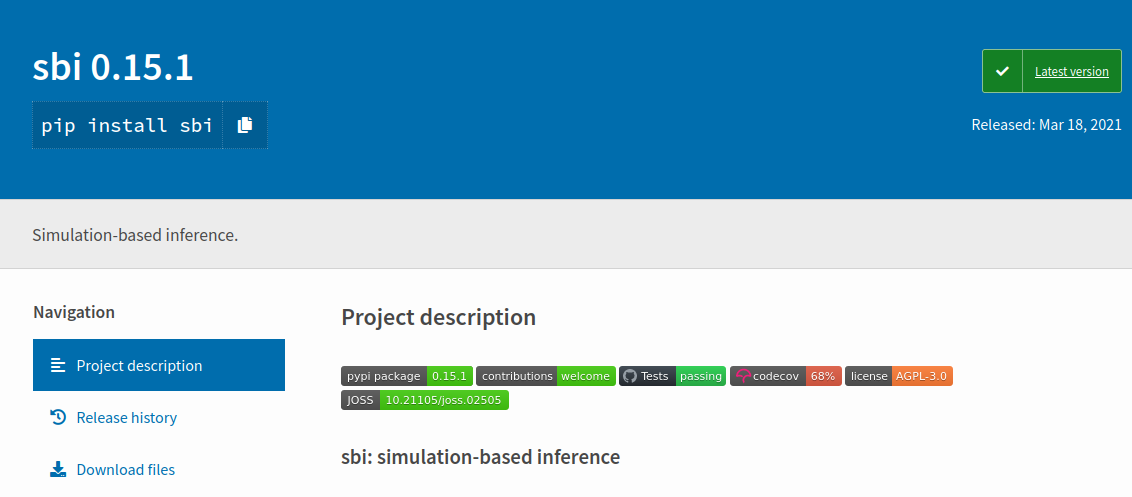
\includegraphics[width=.75\linewidth]{figures/sbipypi.png}
	\end{figure}
\end{itemize}
\end{frame} 


\begin{frame}
\frametitle{References}
\framesubtitle{}
\bibliography{references}
\end{frame} 




\begin{frame}
\frametitle{}
\framesubtitle{}
\begin{itemize}
	\item 
\end{itemize}
\end{frame} 



\end{document}


